%\title{Samosa Recipe}
%\author{Mina Mandal}
%\date{\today}

\maketitle

\begin{figure}[H]
  \centering
  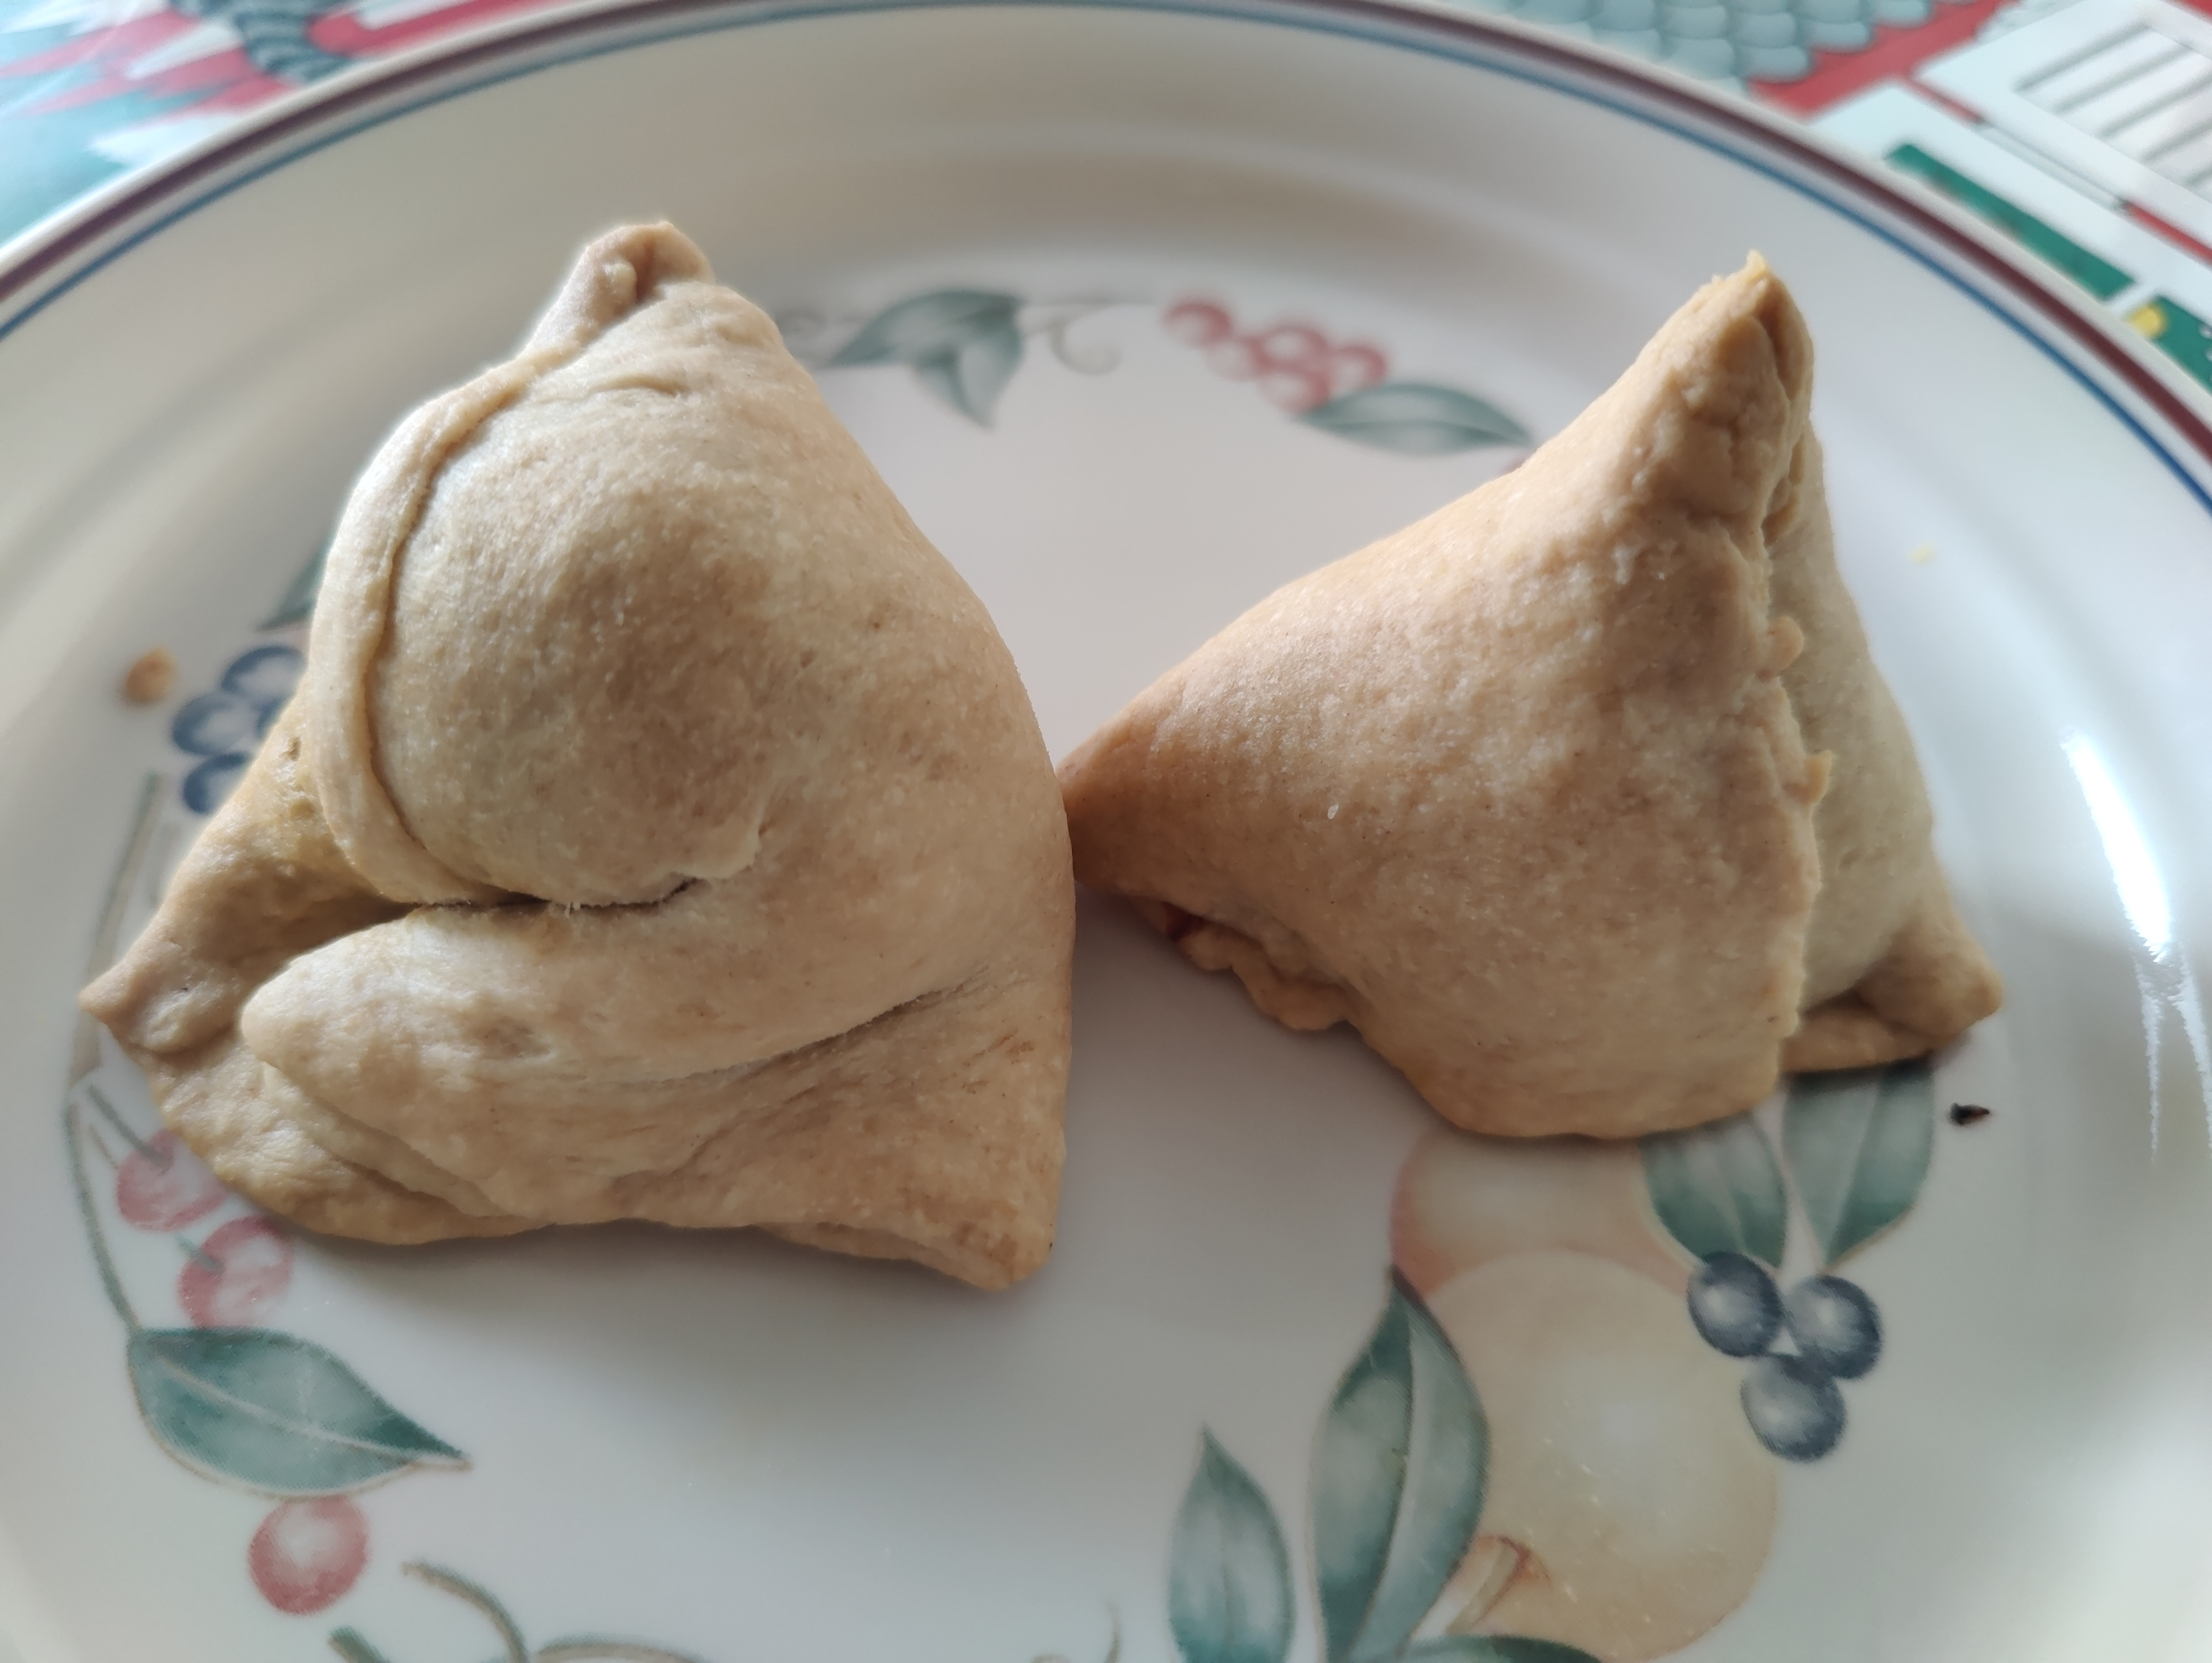
\includegraphics[width=0.5\textwidth]{Samosa/Images/IMG_20231230_154205.jpg}
  \caption{Palm-sized dough ball}
  \label{fig:fig1}
\end{figure}

\section*{Introduction}

These samosas are quite different from regular, traditional Indian samosas. Most samosas are mainly deep fried potatoes. These samosas that my grandma make are instead wrapped with dough, use primarily a cauliflower base, and have a variety of spices, leading to a much more healthy and tasty snack.

\section*{Filling}

\subsection*{Ingredients}
\begin{itemize}
  \item 1x Cauliflower Head
  \item 1x Potato
  \item Vegetable oil
  \item 1/2 cup Peas
  \item 1 1/2 tbsp Salt
  \item 1 tbsp Hot Pepper
  \item 2 tbsp Ginger
  \item 2 tbsp Coriander
  \item 1 1/2 tbsp Cumin
  \item 1 tsp Paprika
\end{itemize}

\subsection*{Instructions}

\begin{enumerate}
  \item Finely dice potato to 1/4 inch chunks.
  \item Put diced potato into a bowl, fill with water, then microwave until soft (\textasciitilde 4 mins at regular power).
  \item Finely chop cauliflower.
  \item Put enough oil in a pan to simmer your cauliflower.
  \item Add cauliflower and bring the pan to a simmer.
  \item Drain water from potatoes, then add the potatoes to the pan.
  \item Add salt, hot pepper, ginger, coriander, cumin, and paprika.
  \item Add 1 tbsp oil and stir, mash the bigger pieces down.
  \item Add 1 tsp garam masala.
  \item Add 1/2 cup peas.
  \item Bring the temperature down to low and cover.
  \item If your mix is watery, add 4 tbsp of potato flakes. Starch can be used as an alternative.
\end{enumerate}

\section*{Dough}

\begin{itemize}
  \item 2 cups of bleached, self-rising flour
  \item 1/2 cup vegetable shortening
  \item 1/2 - 3/4 cups warm water
\end{itemize}

\subsection*{Instructions}

\begin{enumerate}
  \item Add flour to a bowl.
  \item Knead shortening into flour.
  \item Slowly mix in water. Knead until there is a doughy consistency.
  \item Separate into palm-sized balls (see Figure \ref{fig:fig1}).
\end{enumerate}

\begin{figure}[H]
  \centering
  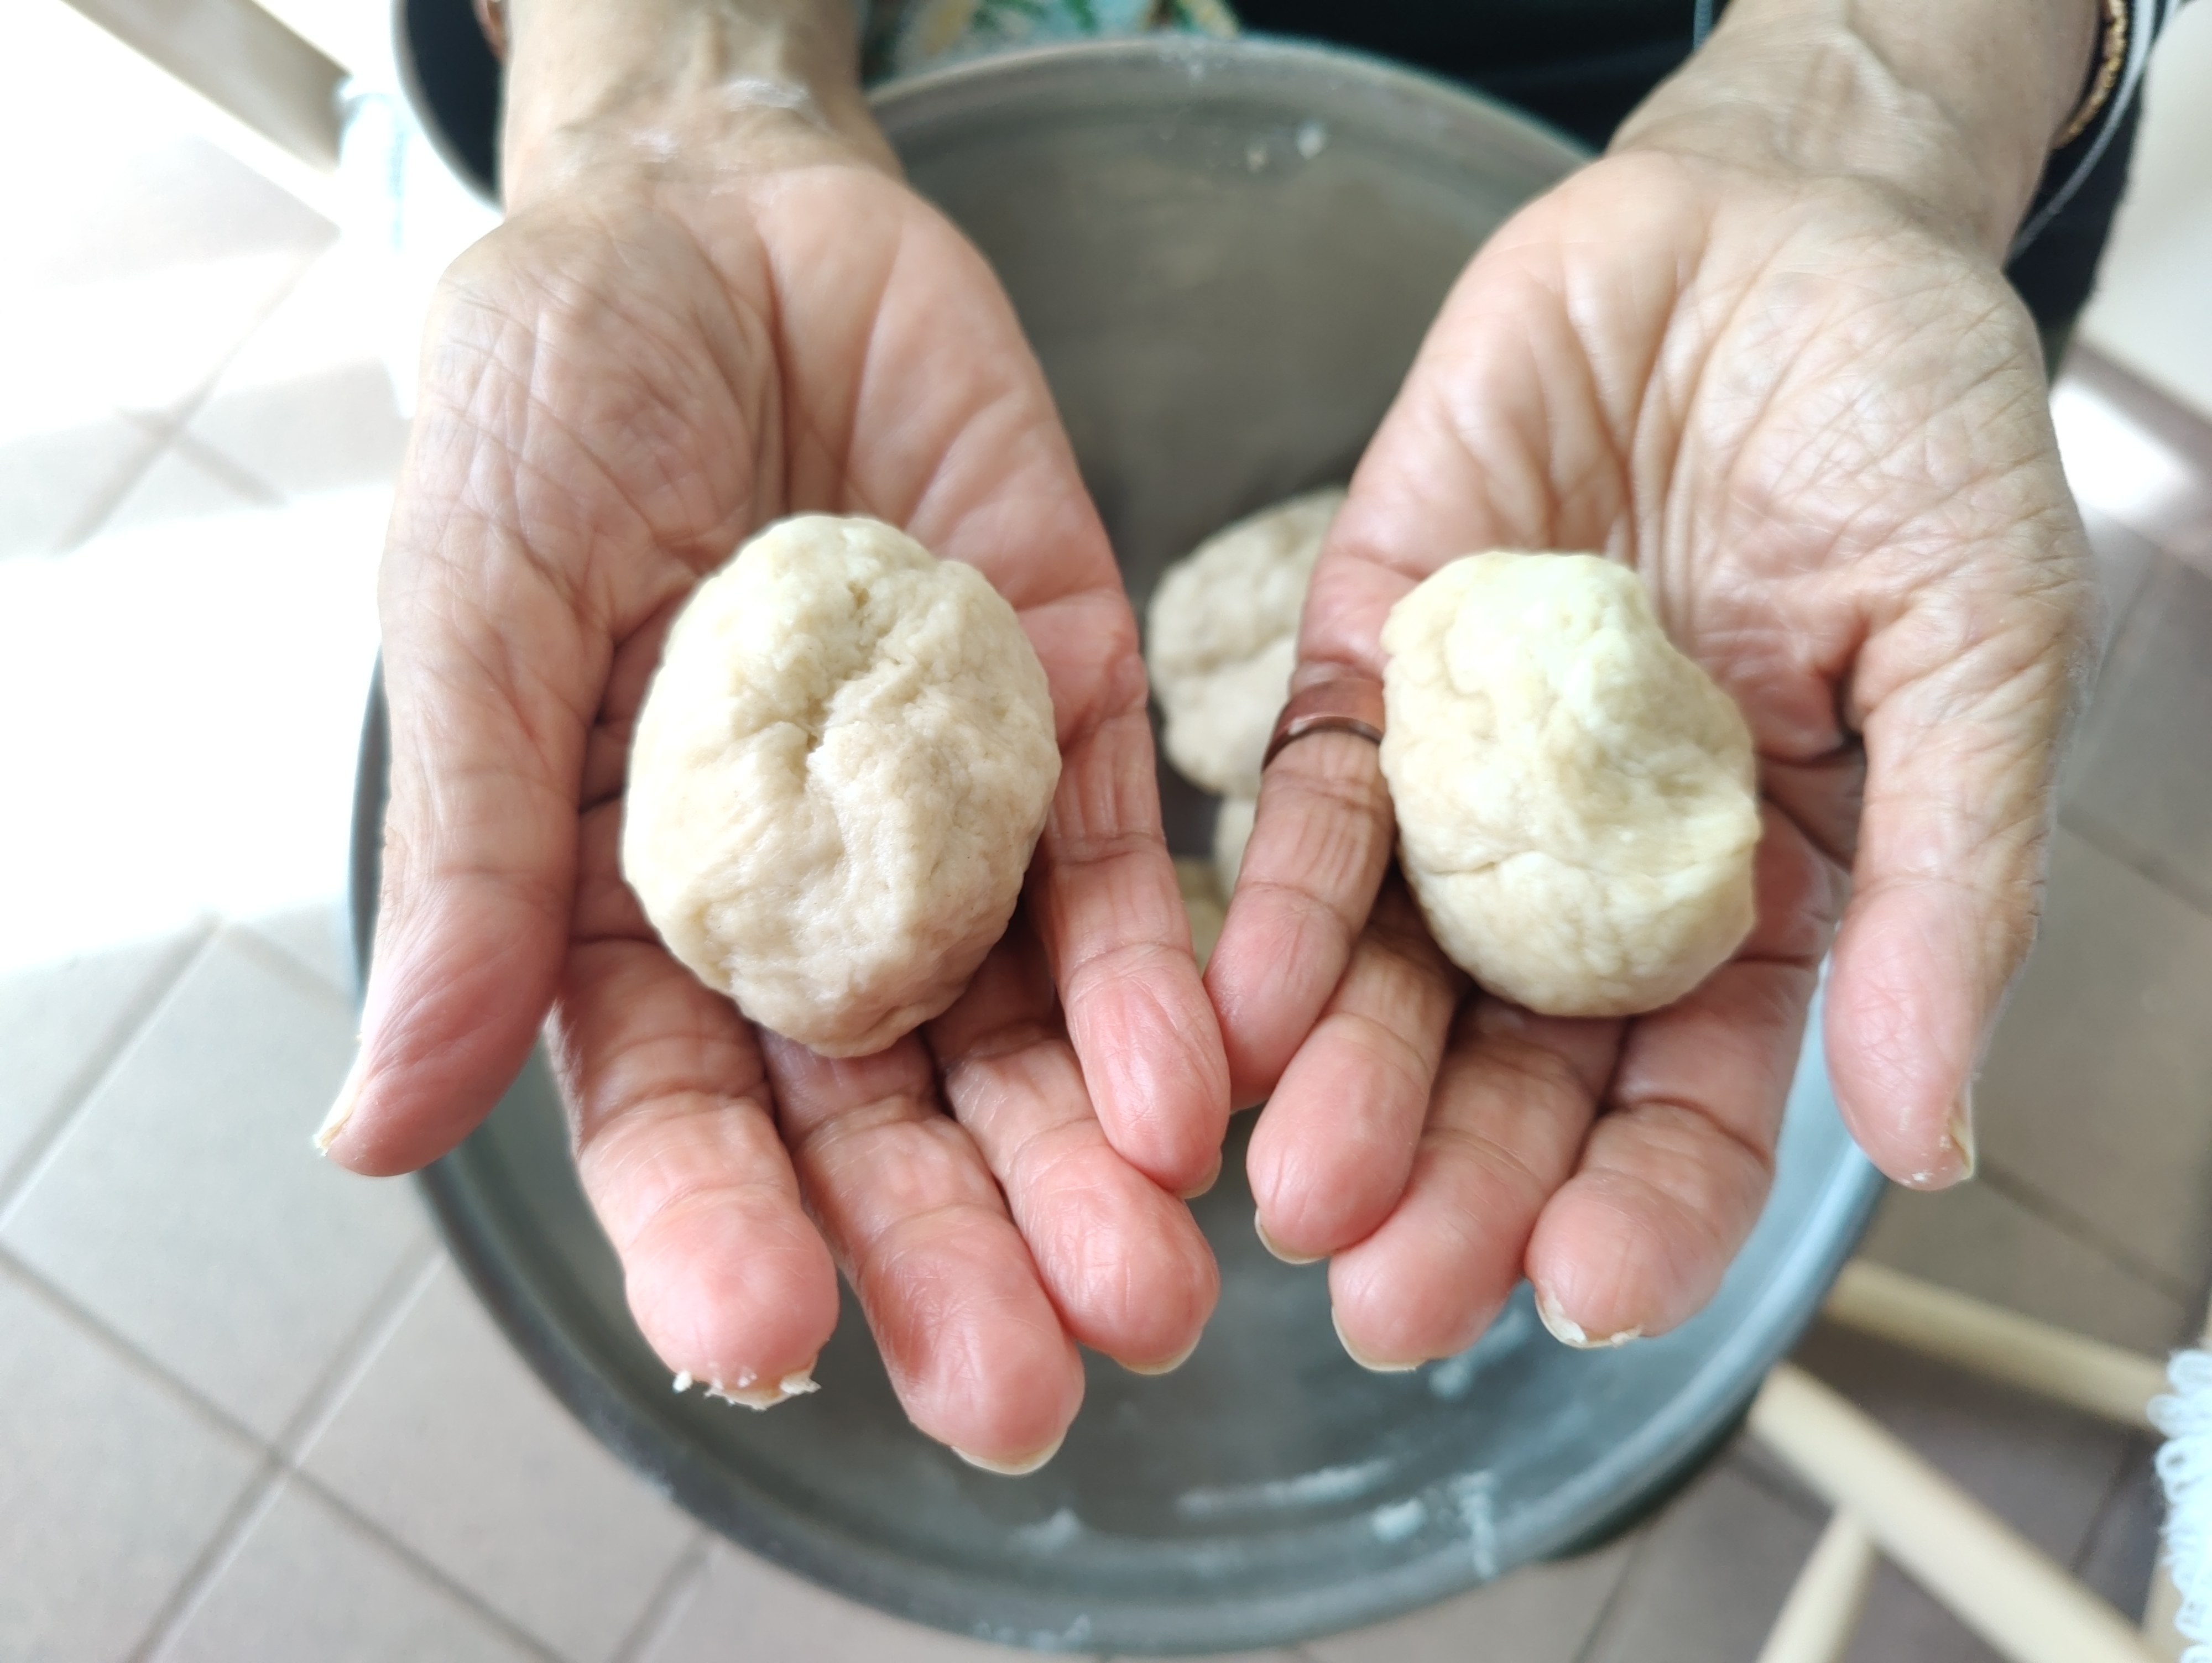
\includegraphics[width=0.5\textwidth]{Samosa/Images/IMG_20231230_142118.jpg}
  \caption{Palm-sized dough ball}
  \label{fig:fig1}
\end{figure}

\section*{Making the Samosas}

\begin{enumerate}
  \item Get a baking sheet, cover it with parchment paper. Preheat oven to 270 F
  \item Push the dough ball into a disk, cover the disk and surface with flour.
  \item Roll the dough disk so it is oblong. Cut the dough disk into two across the short distance.
  \item Fold into a cone along the cut edge.
  \item Fill the cone with the prepared filling.
  \item Pinch the opposite side of the folded crease, fold into the opposite side, then push the edges together.
  \item Set on the baking sheet.
  \item Bake until edges are slightly brown (\textasciitilde 20 minutes). Then raise temperature to 300 F on convect.
\end{enumerate}

\begin{figure}[H]
  \centering
  \begin{subfigure}[b]{0.3\textwidth}
    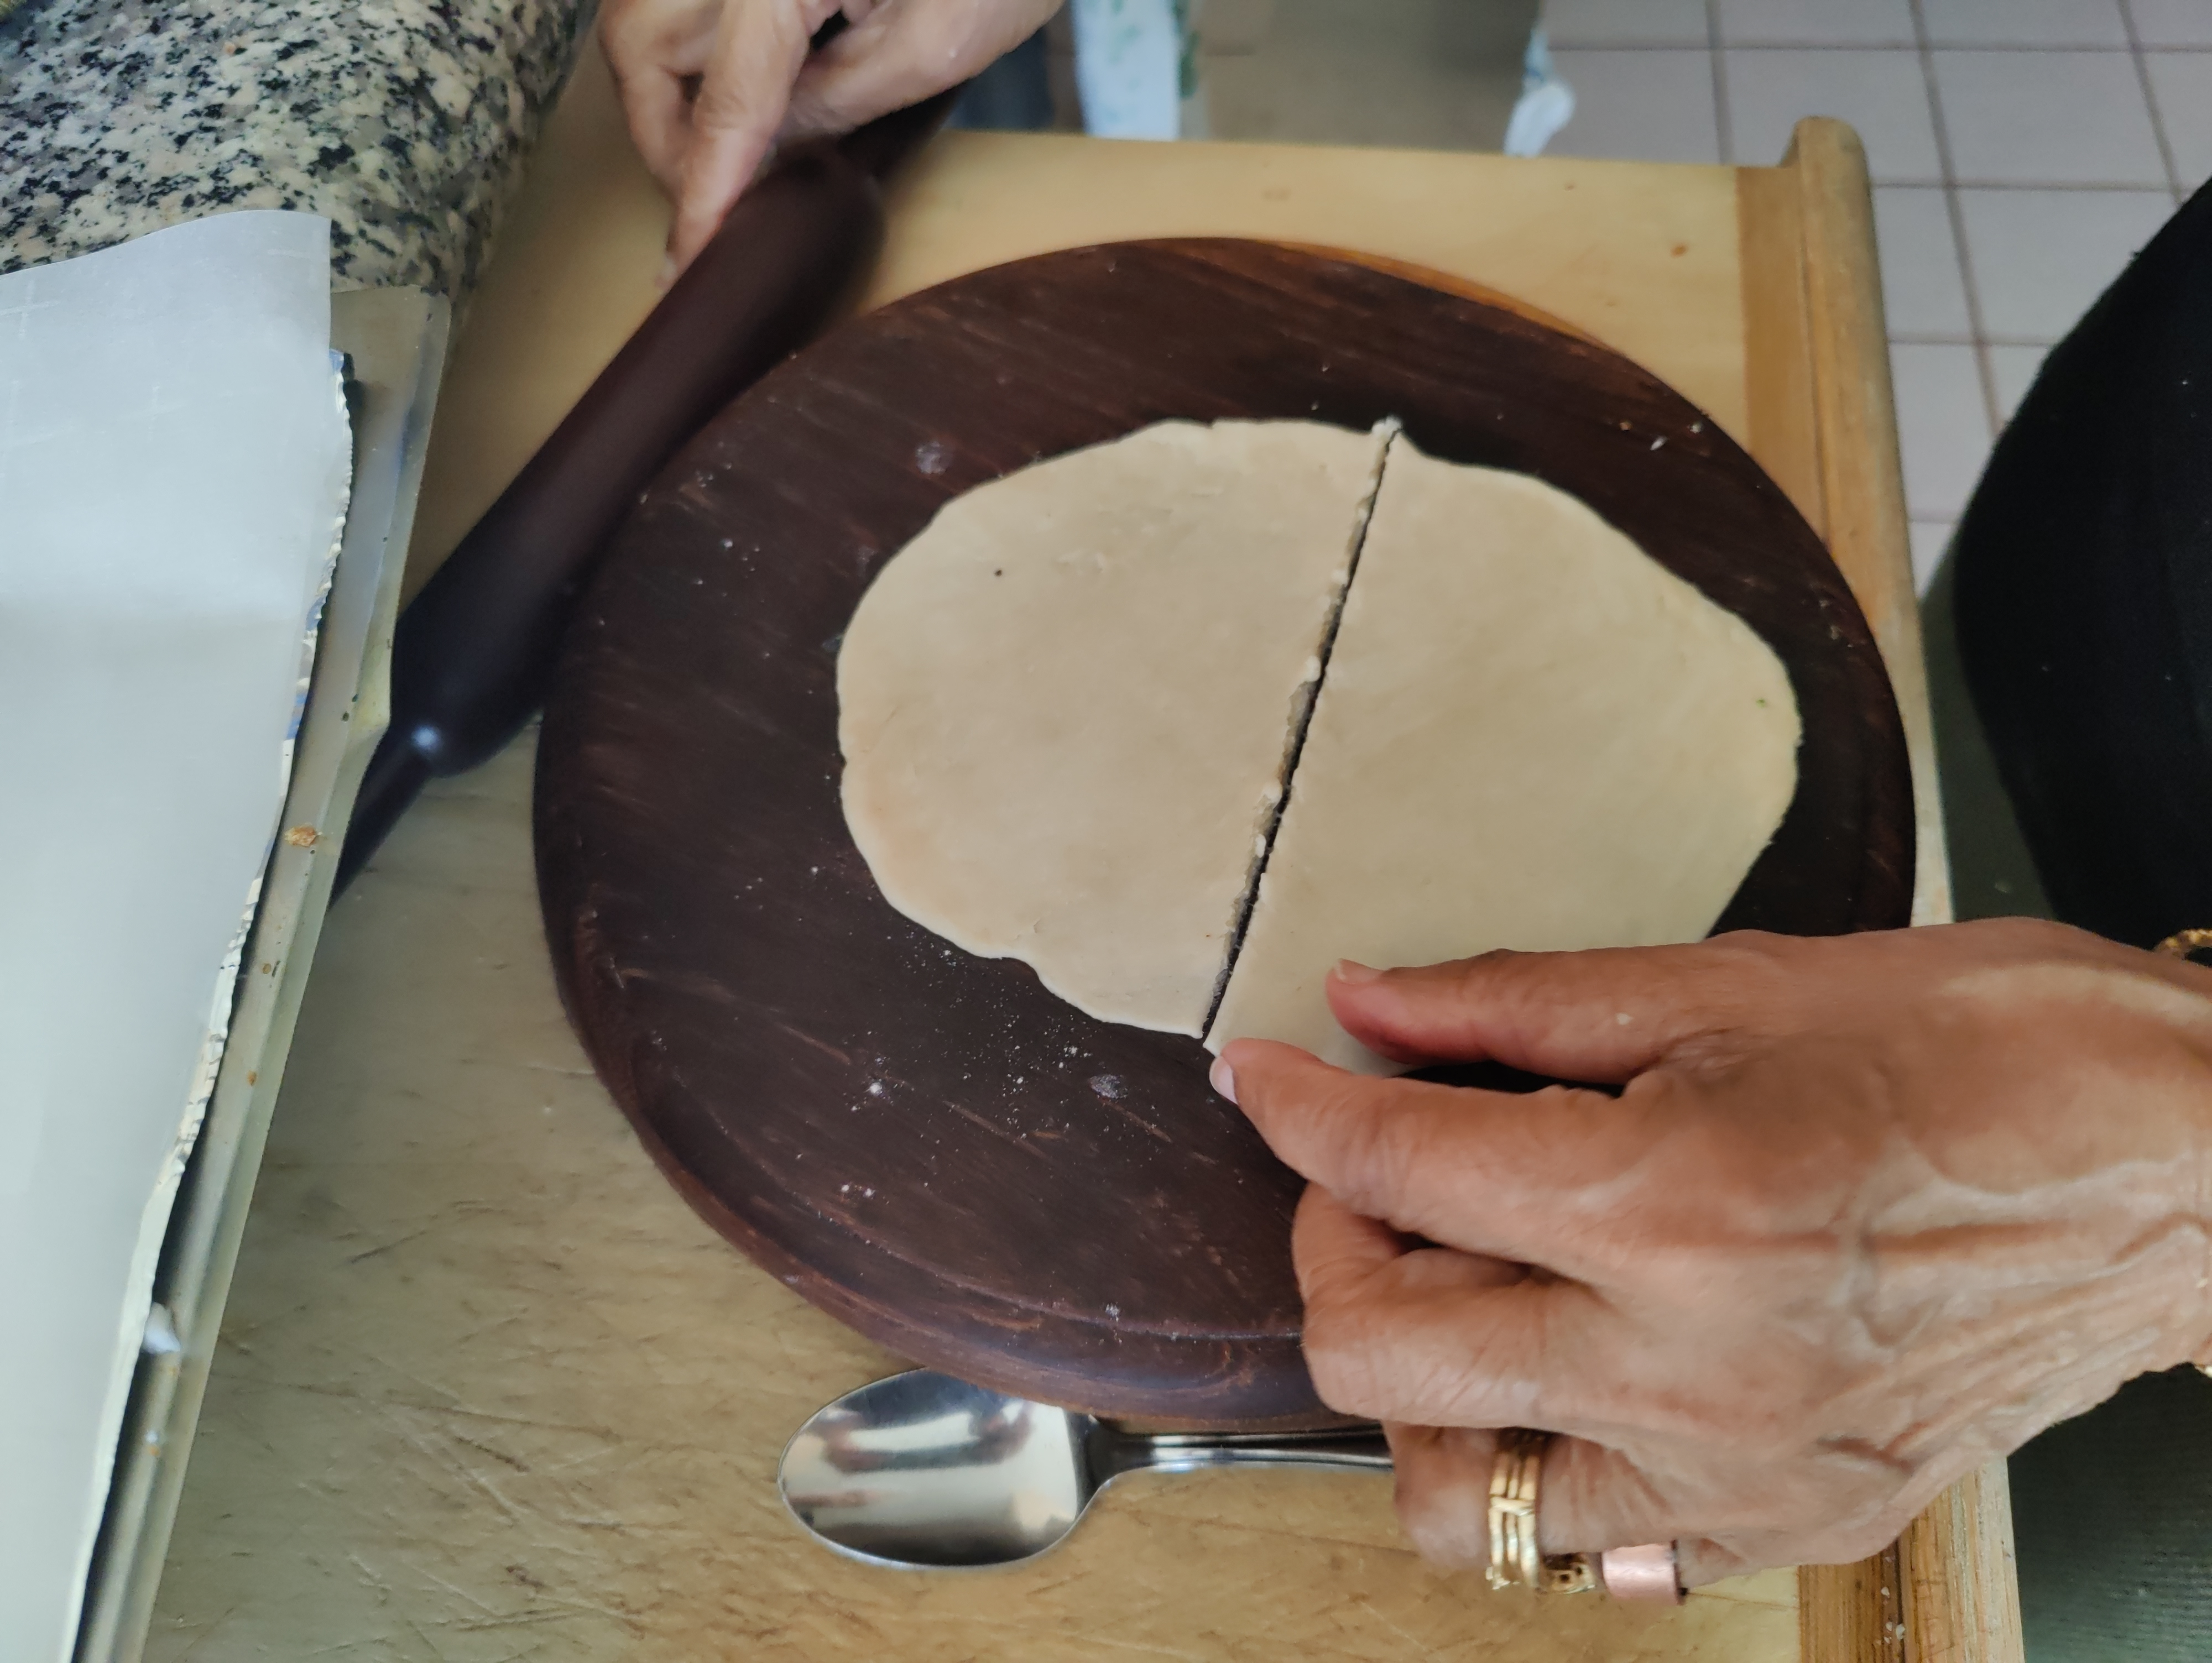
\includegraphics[width=\textwidth]{Samosa/Images/IMG_20231230_143632.jpg}
    \caption{Roll oblong and slice}
  \end{subfigure}
  \hfill
  \begin{subfigure}[b]{0.3\textwidth}
    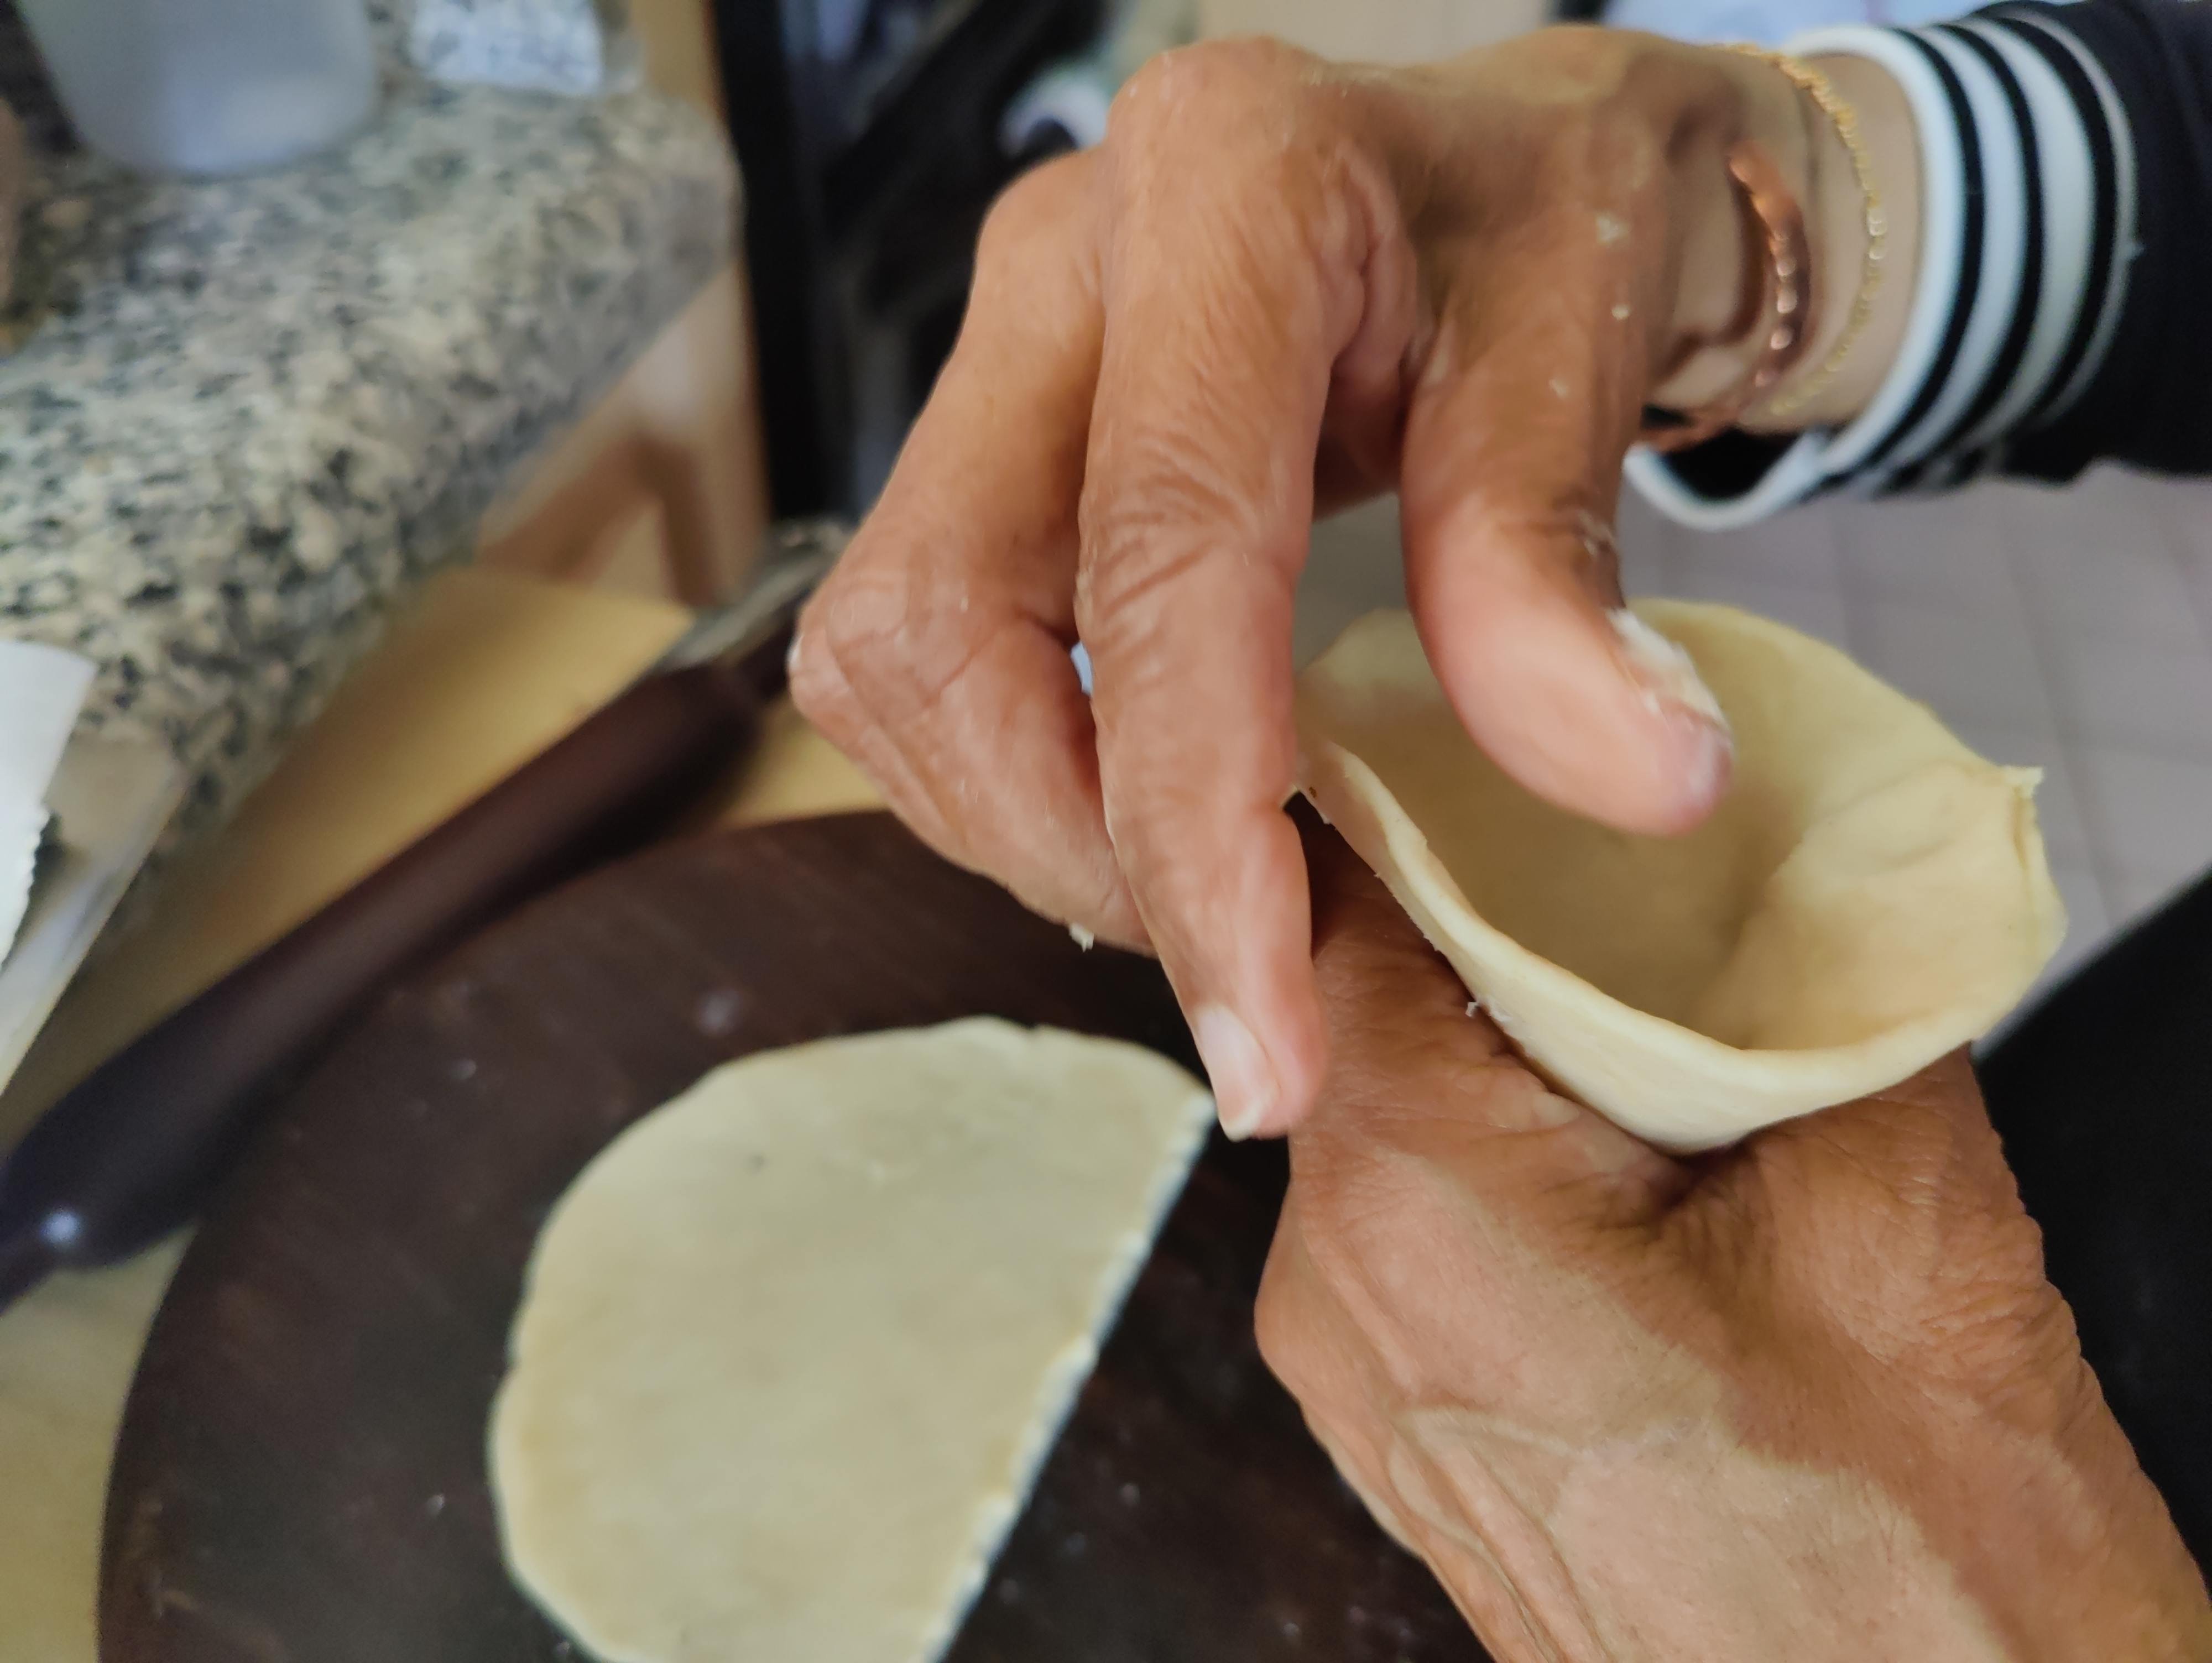
\includegraphics[width=\textwidth]{Samosa/Images/IMG_20231230_143649.jpg}
    \caption{Fold along cut edge}
  \end{subfigure}
  \begin{subfigure}[b]{0.3\textwidth}
    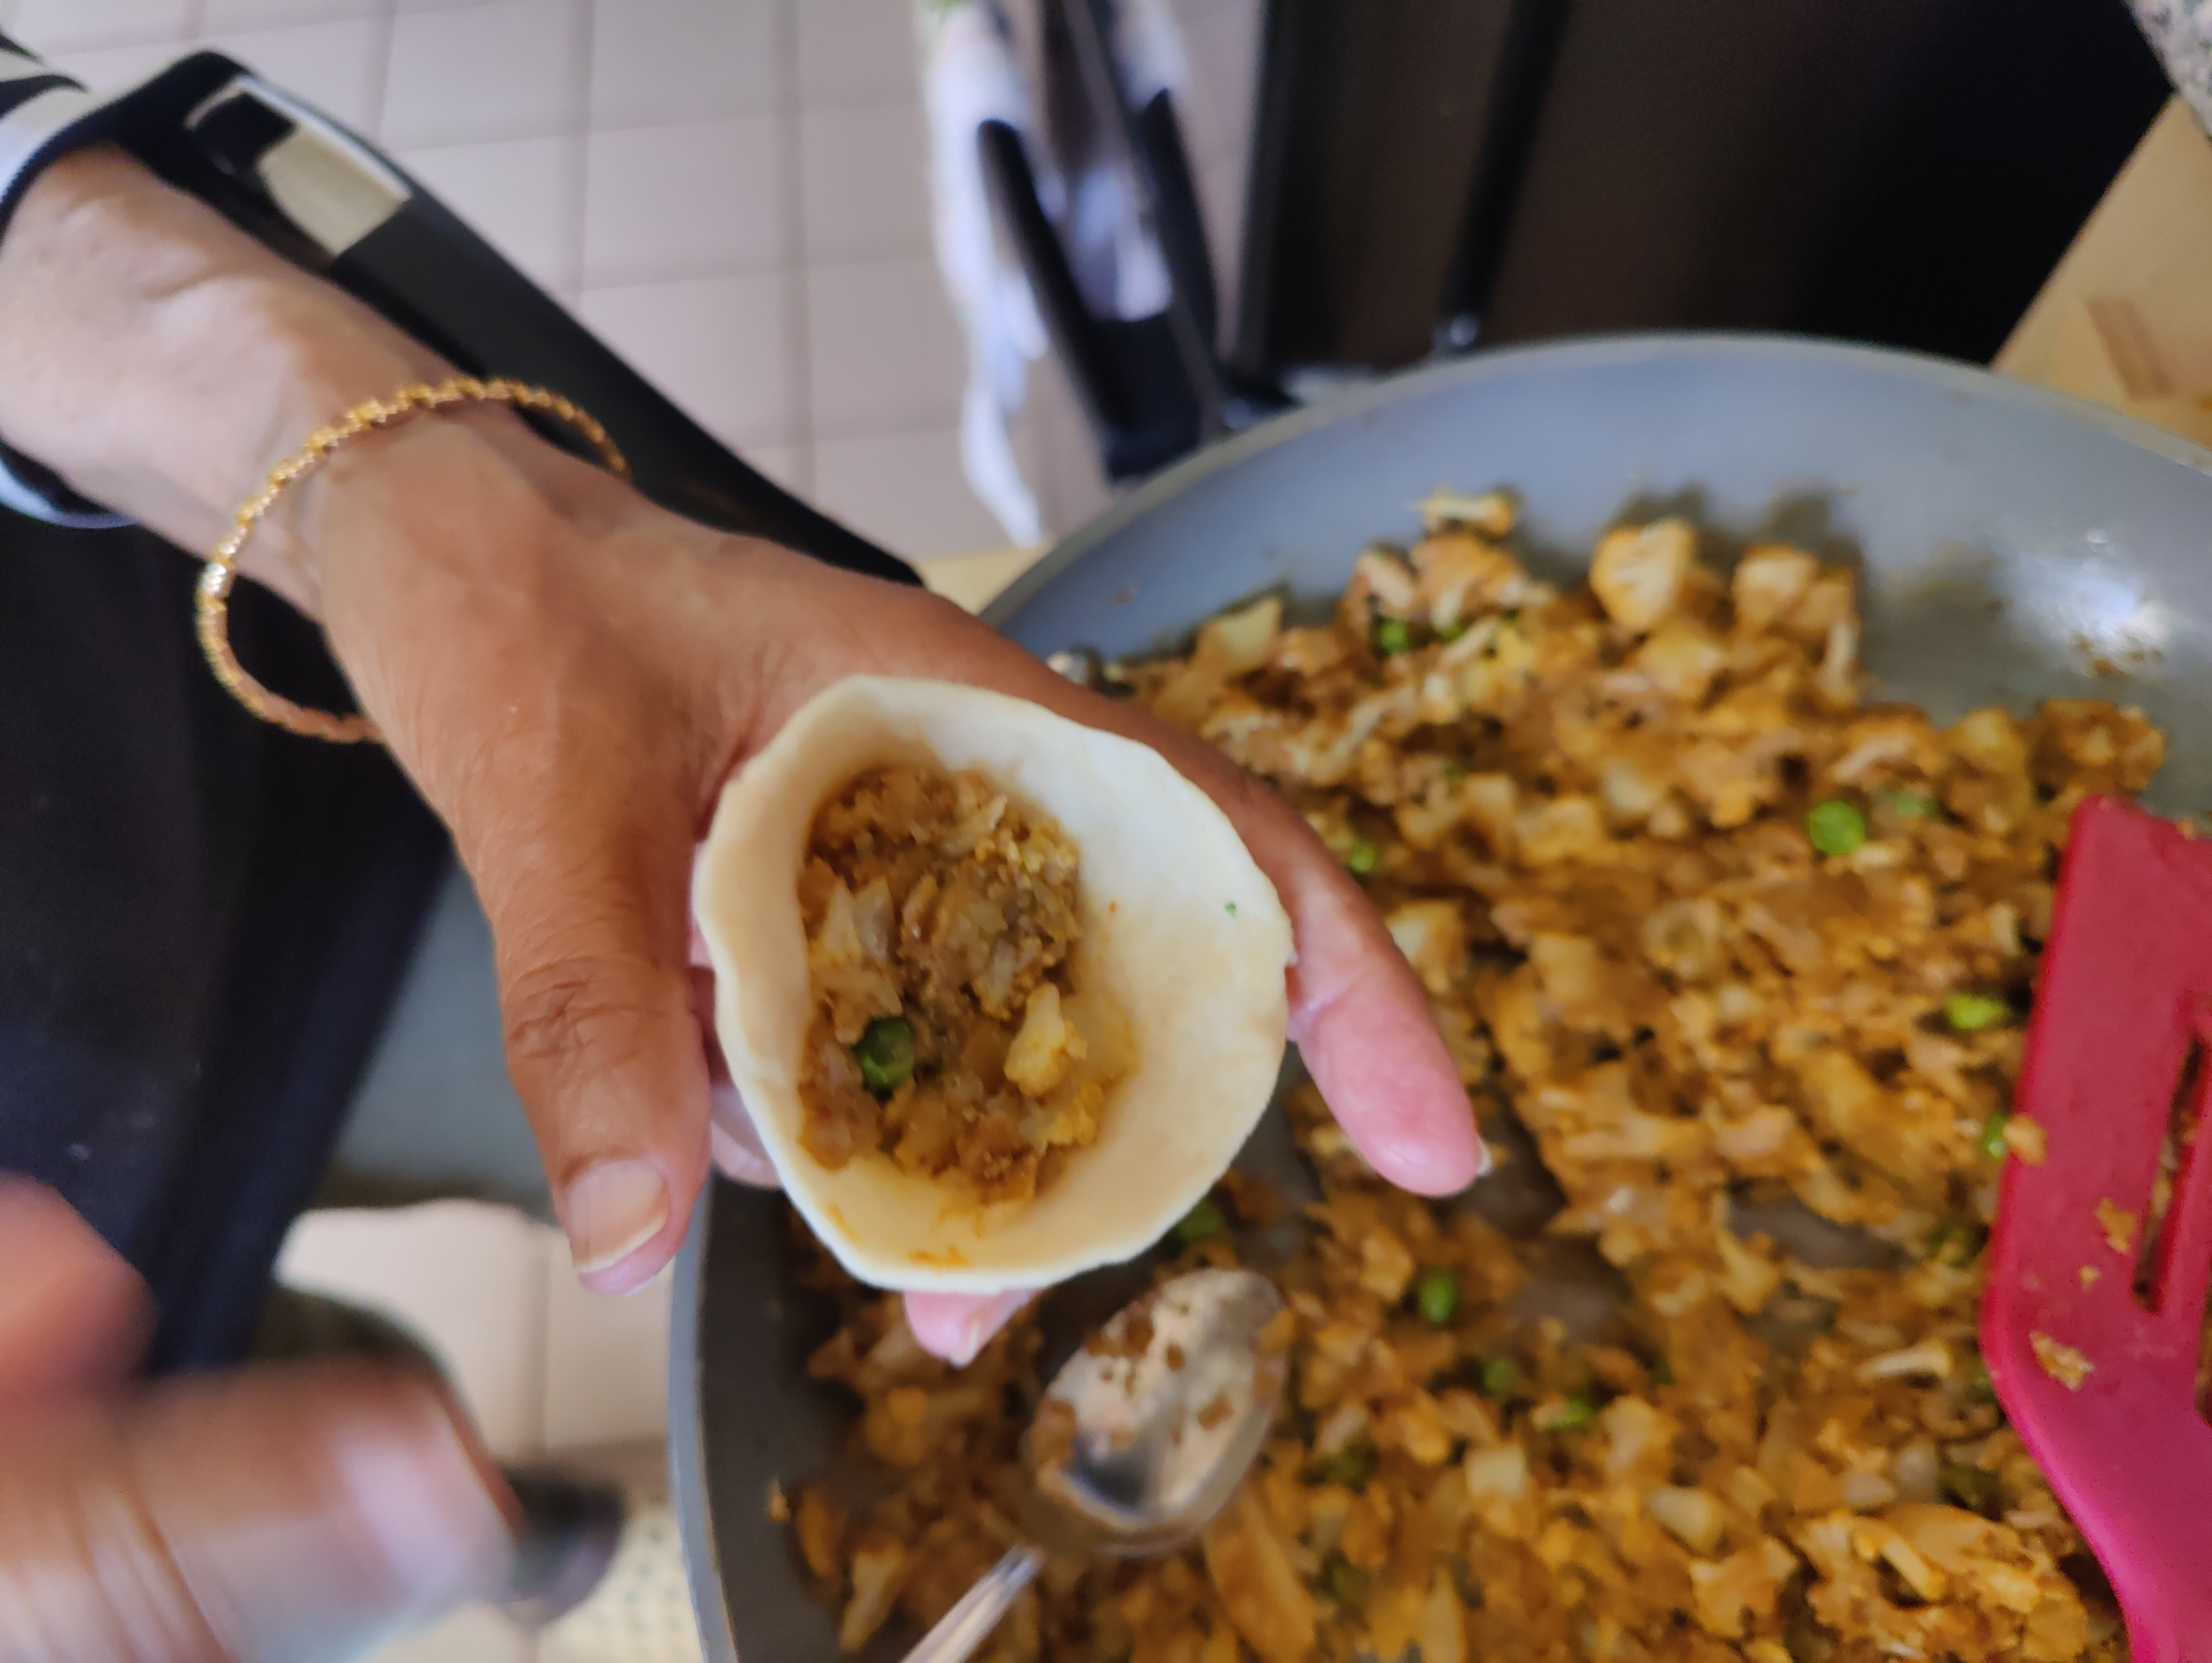
\includegraphics[width=\textwidth]{Samosa/Images/IMG_20231230_143723.jpg}
    \caption{Fill Cone}
  \end{subfigure}
  
  \medskip % Add some space between the rows

  \begin{subfigure}[b]{0.3\textwidth}
    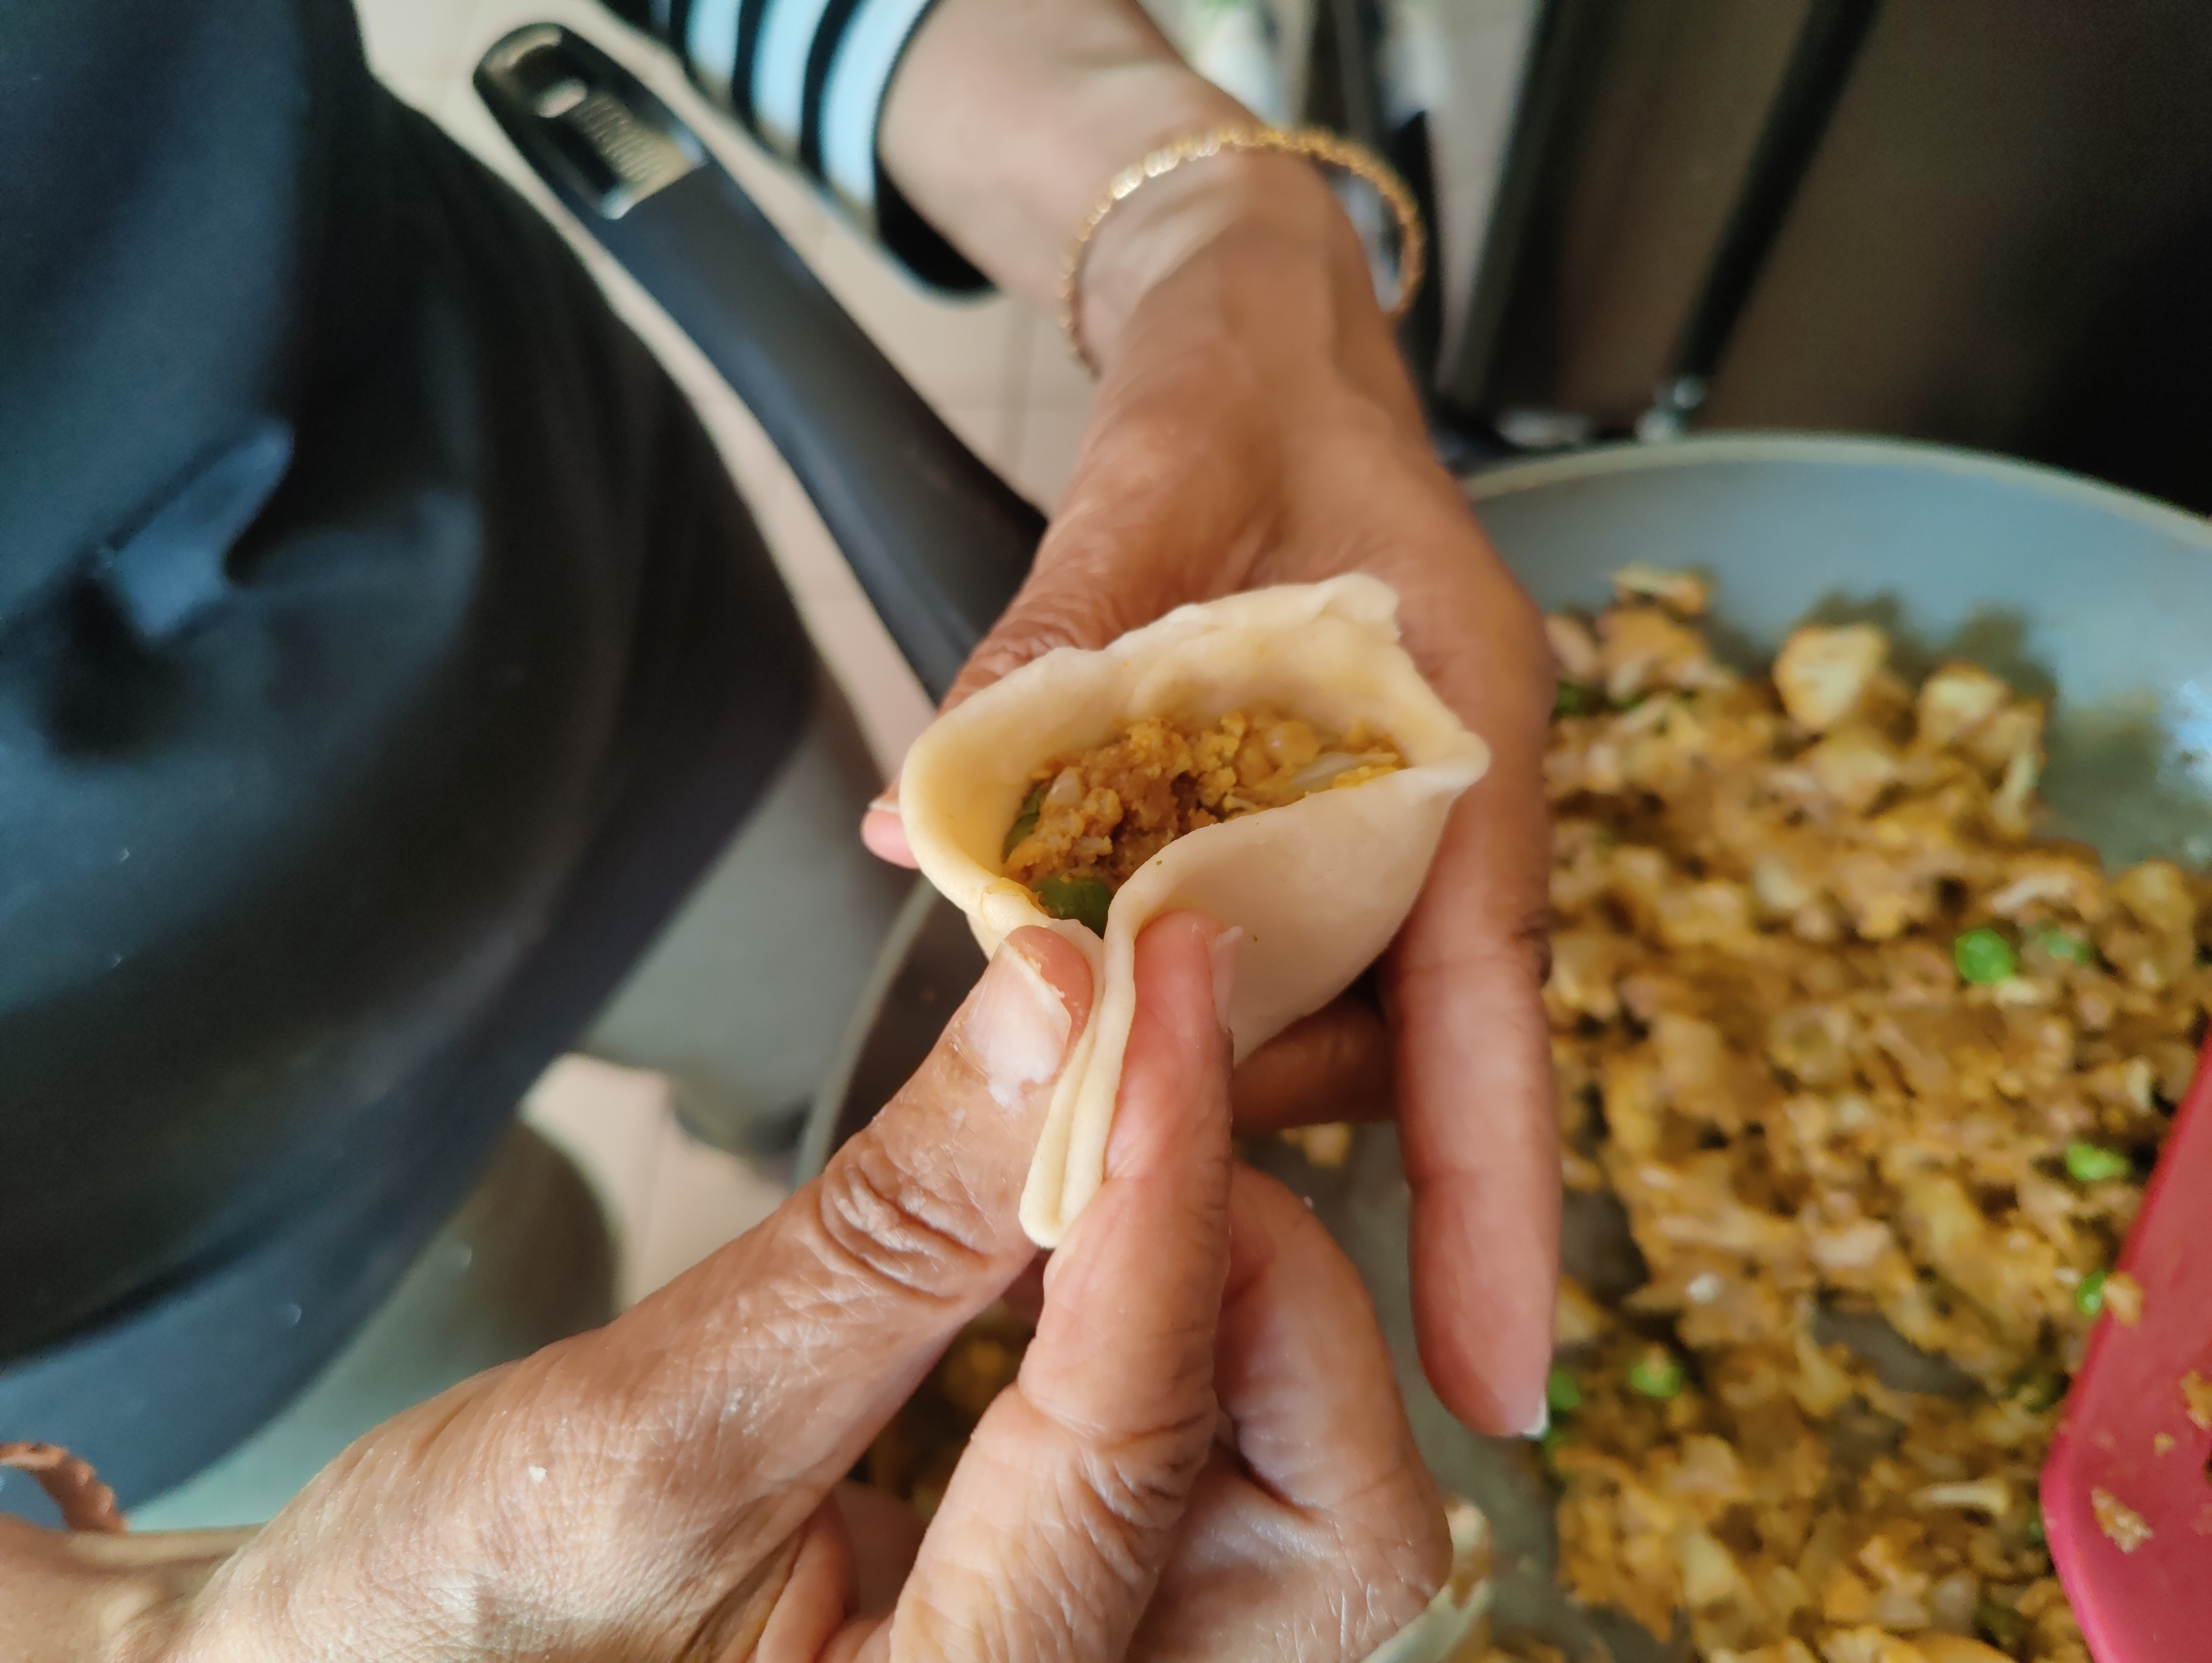
\includegraphics[width=\textwidth]{Samosa/Images/IMG_20231230_143831.jpg}
    \caption{Pinch opposite side}
  \end{subfigure}
  \hfill
  \begin{subfigure}{0.3\textwidth}
    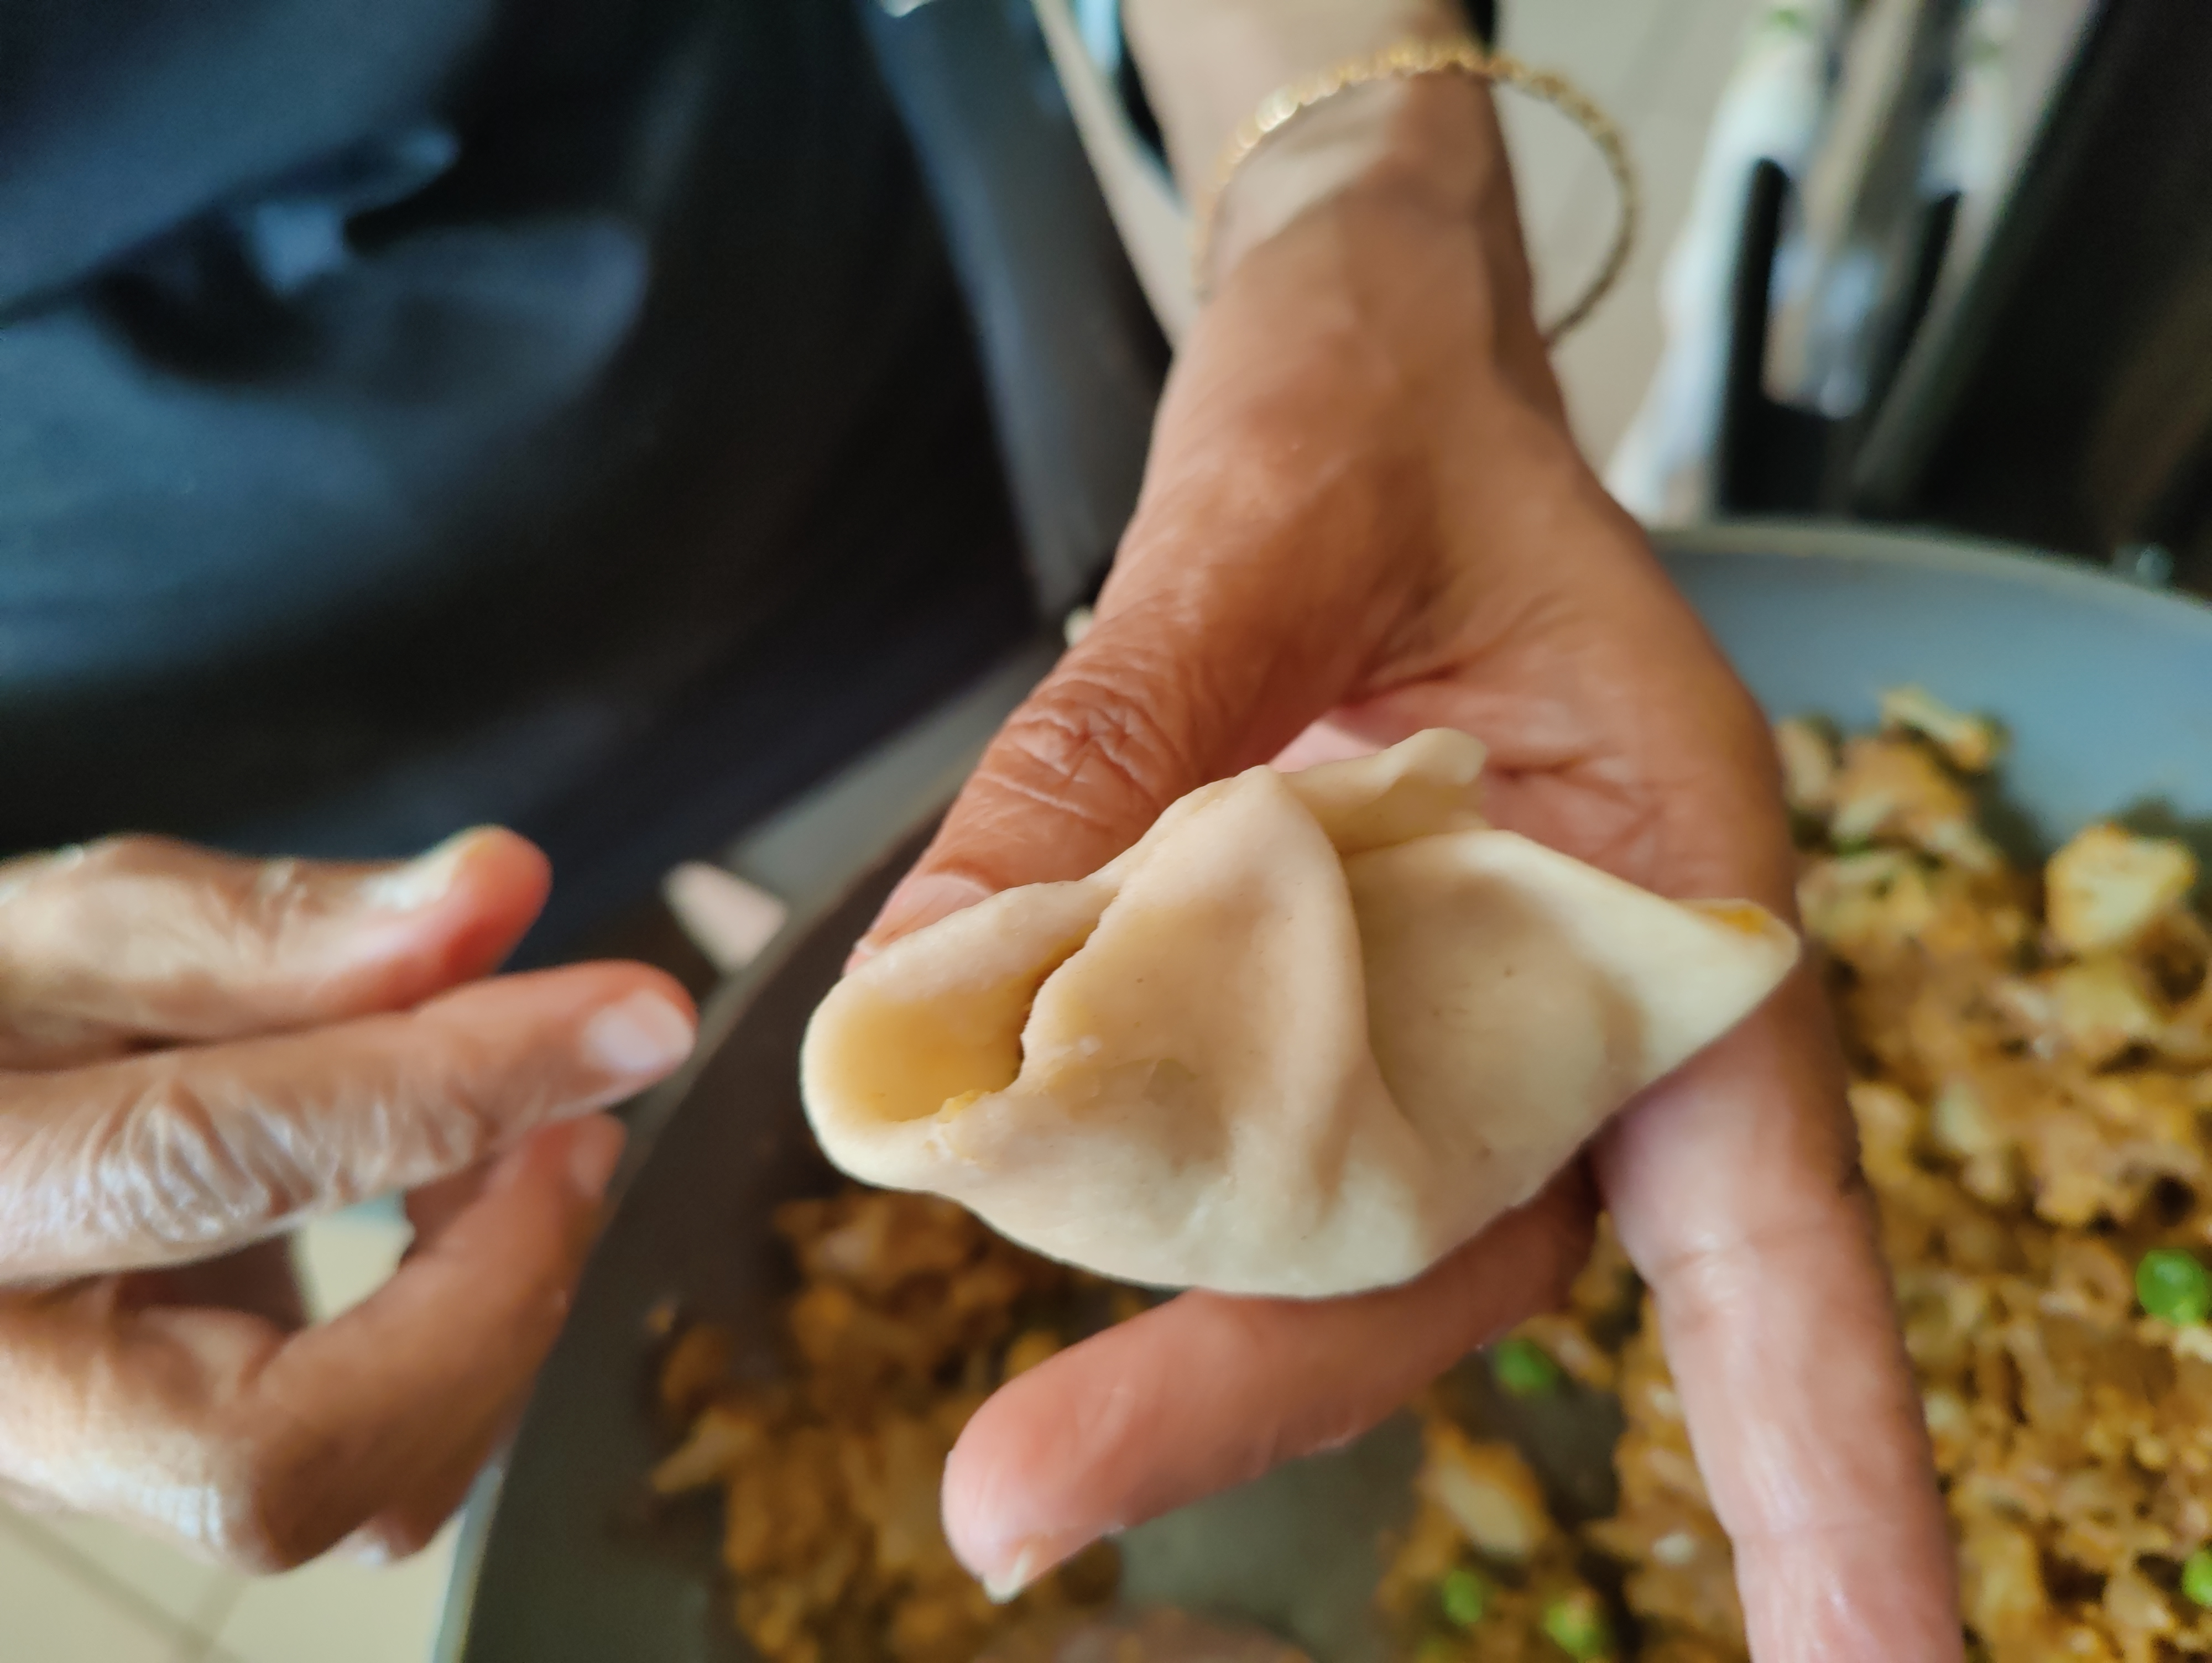
\includegraphics[width=\linewidth]{Samosa/Images/IMG_20231230_143841.jpg}
    \caption{Pinch together}
  \end{subfigure}
  \hfill
  \begin{subfigure}{0.3\textwidth}
    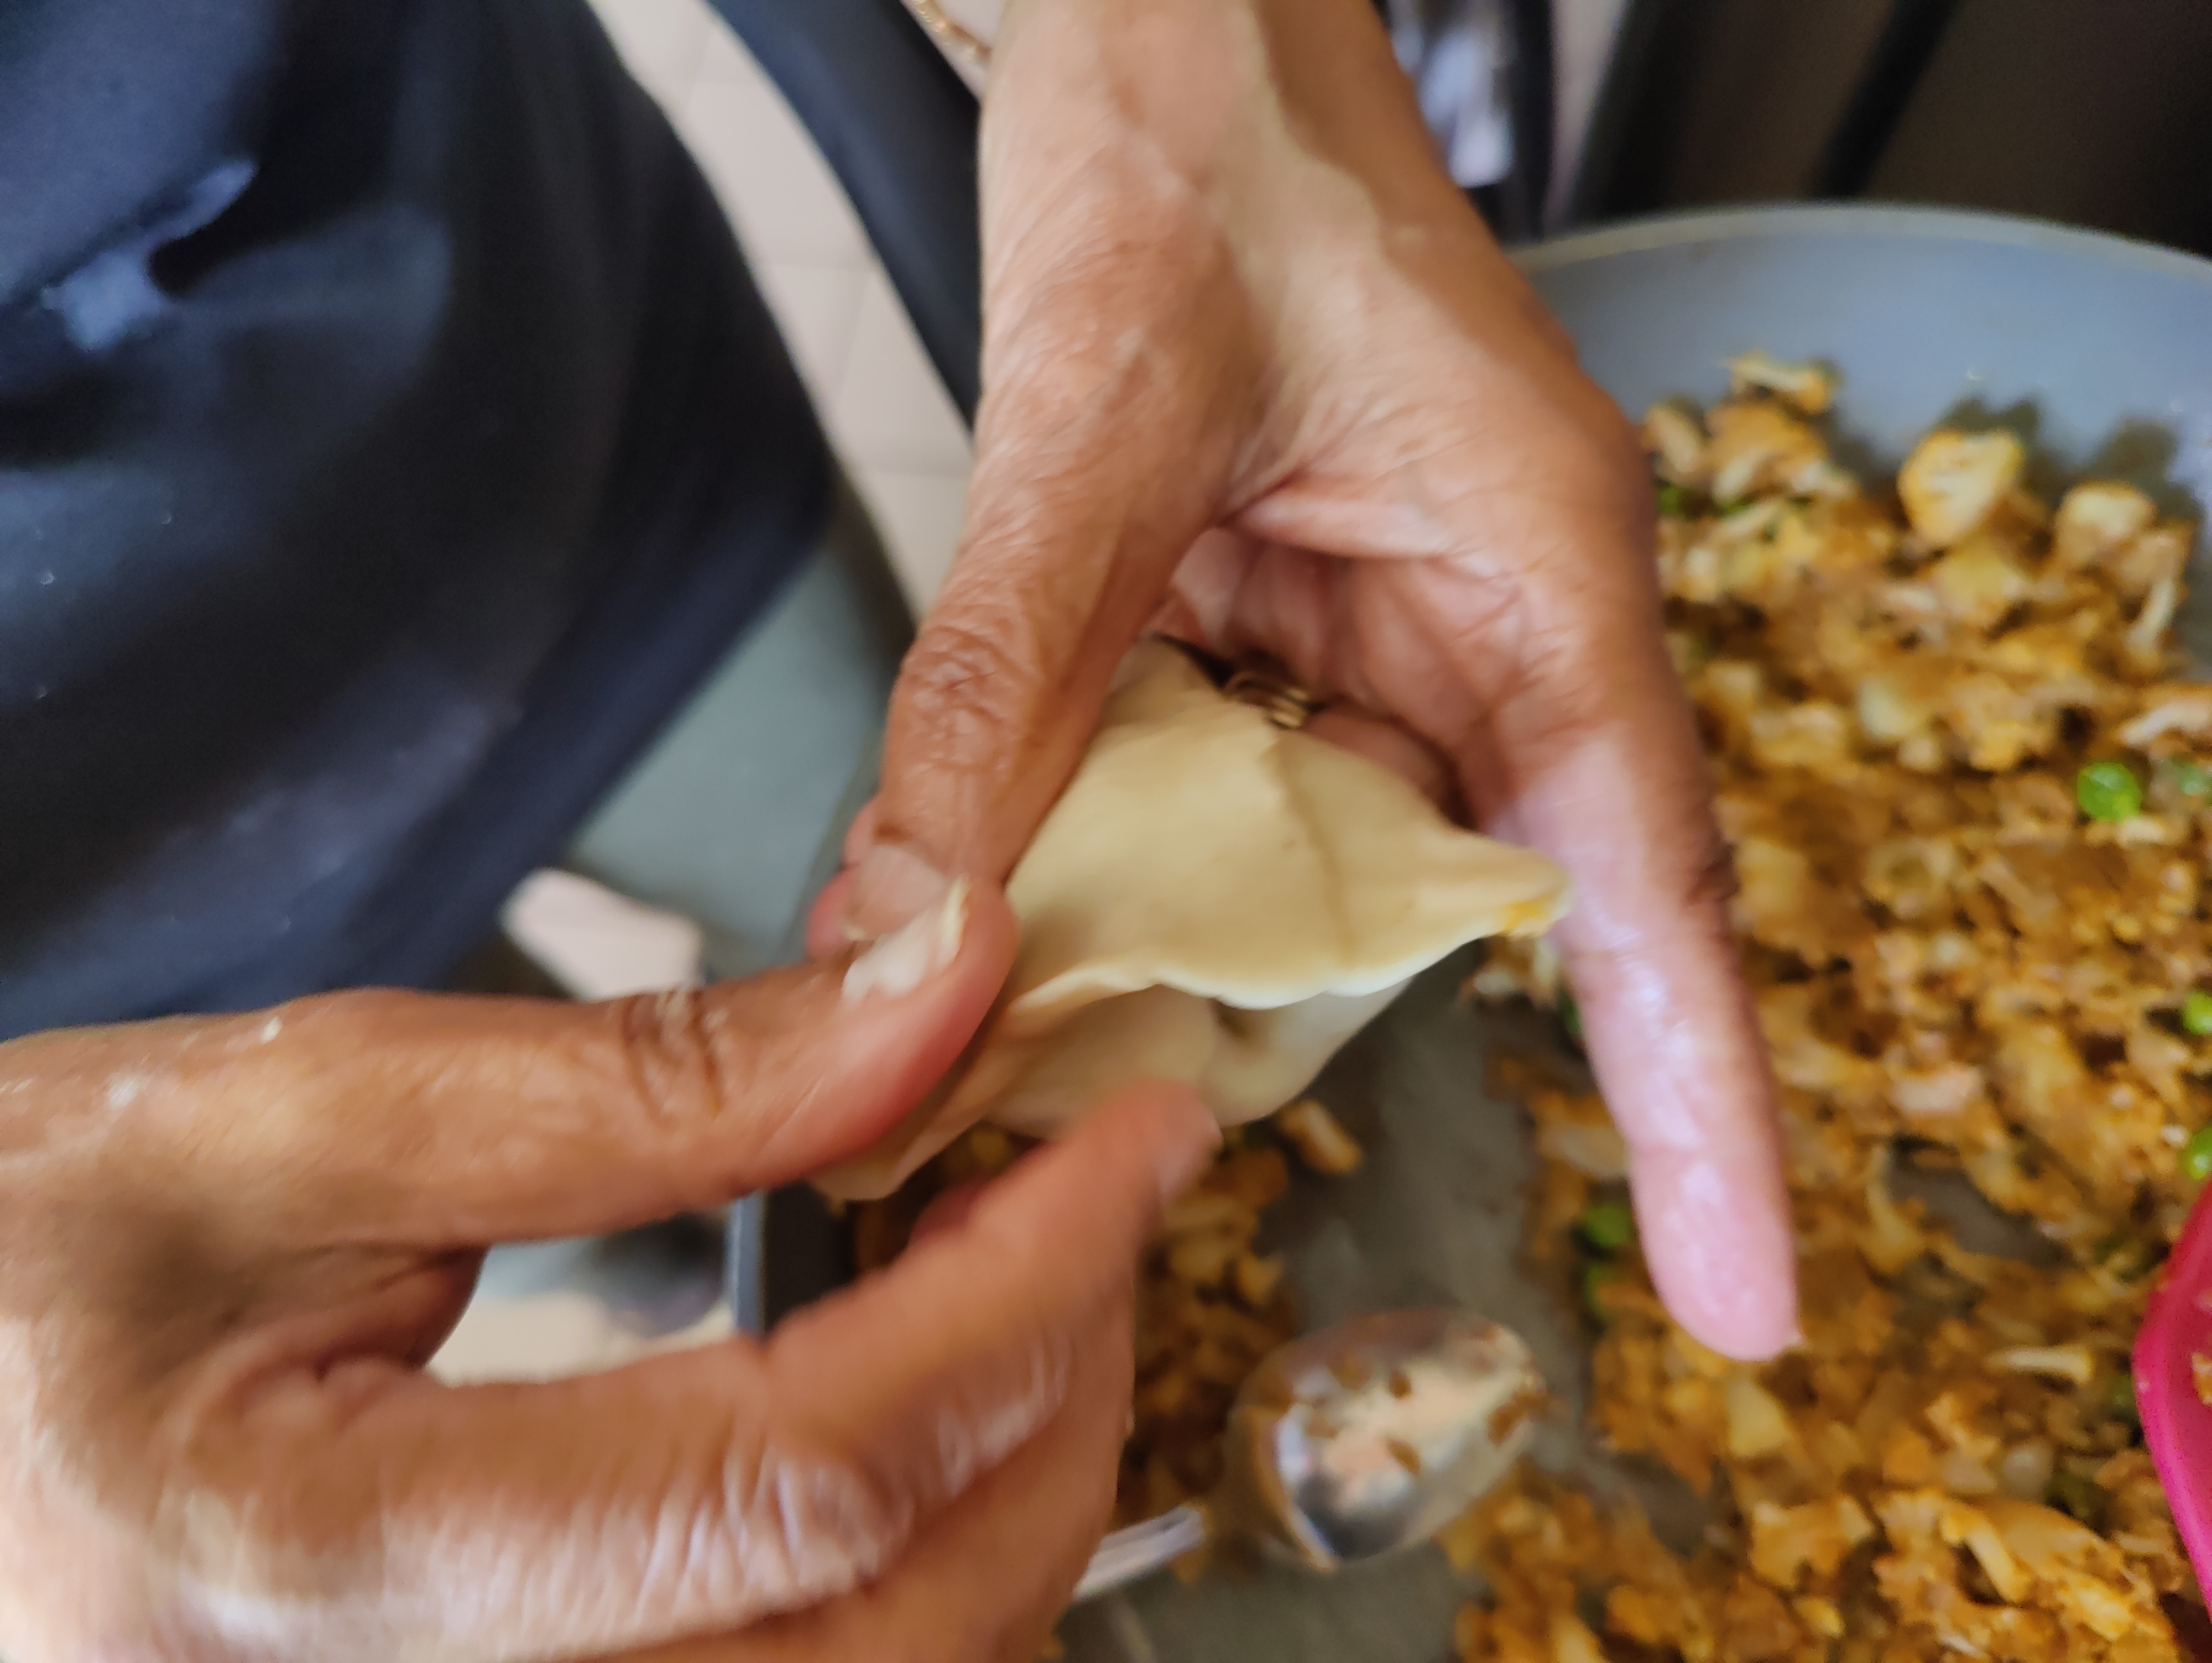
\includegraphics[width=\linewidth]{Samosa/Images/IMG_20231230_143850.jpg}
    \caption{Close samosa}
  \end{subfigure}

  \caption{Folding Process}
  \label{fig:folds}
\end{figure}

\begin{figure}[H]
  \centering
  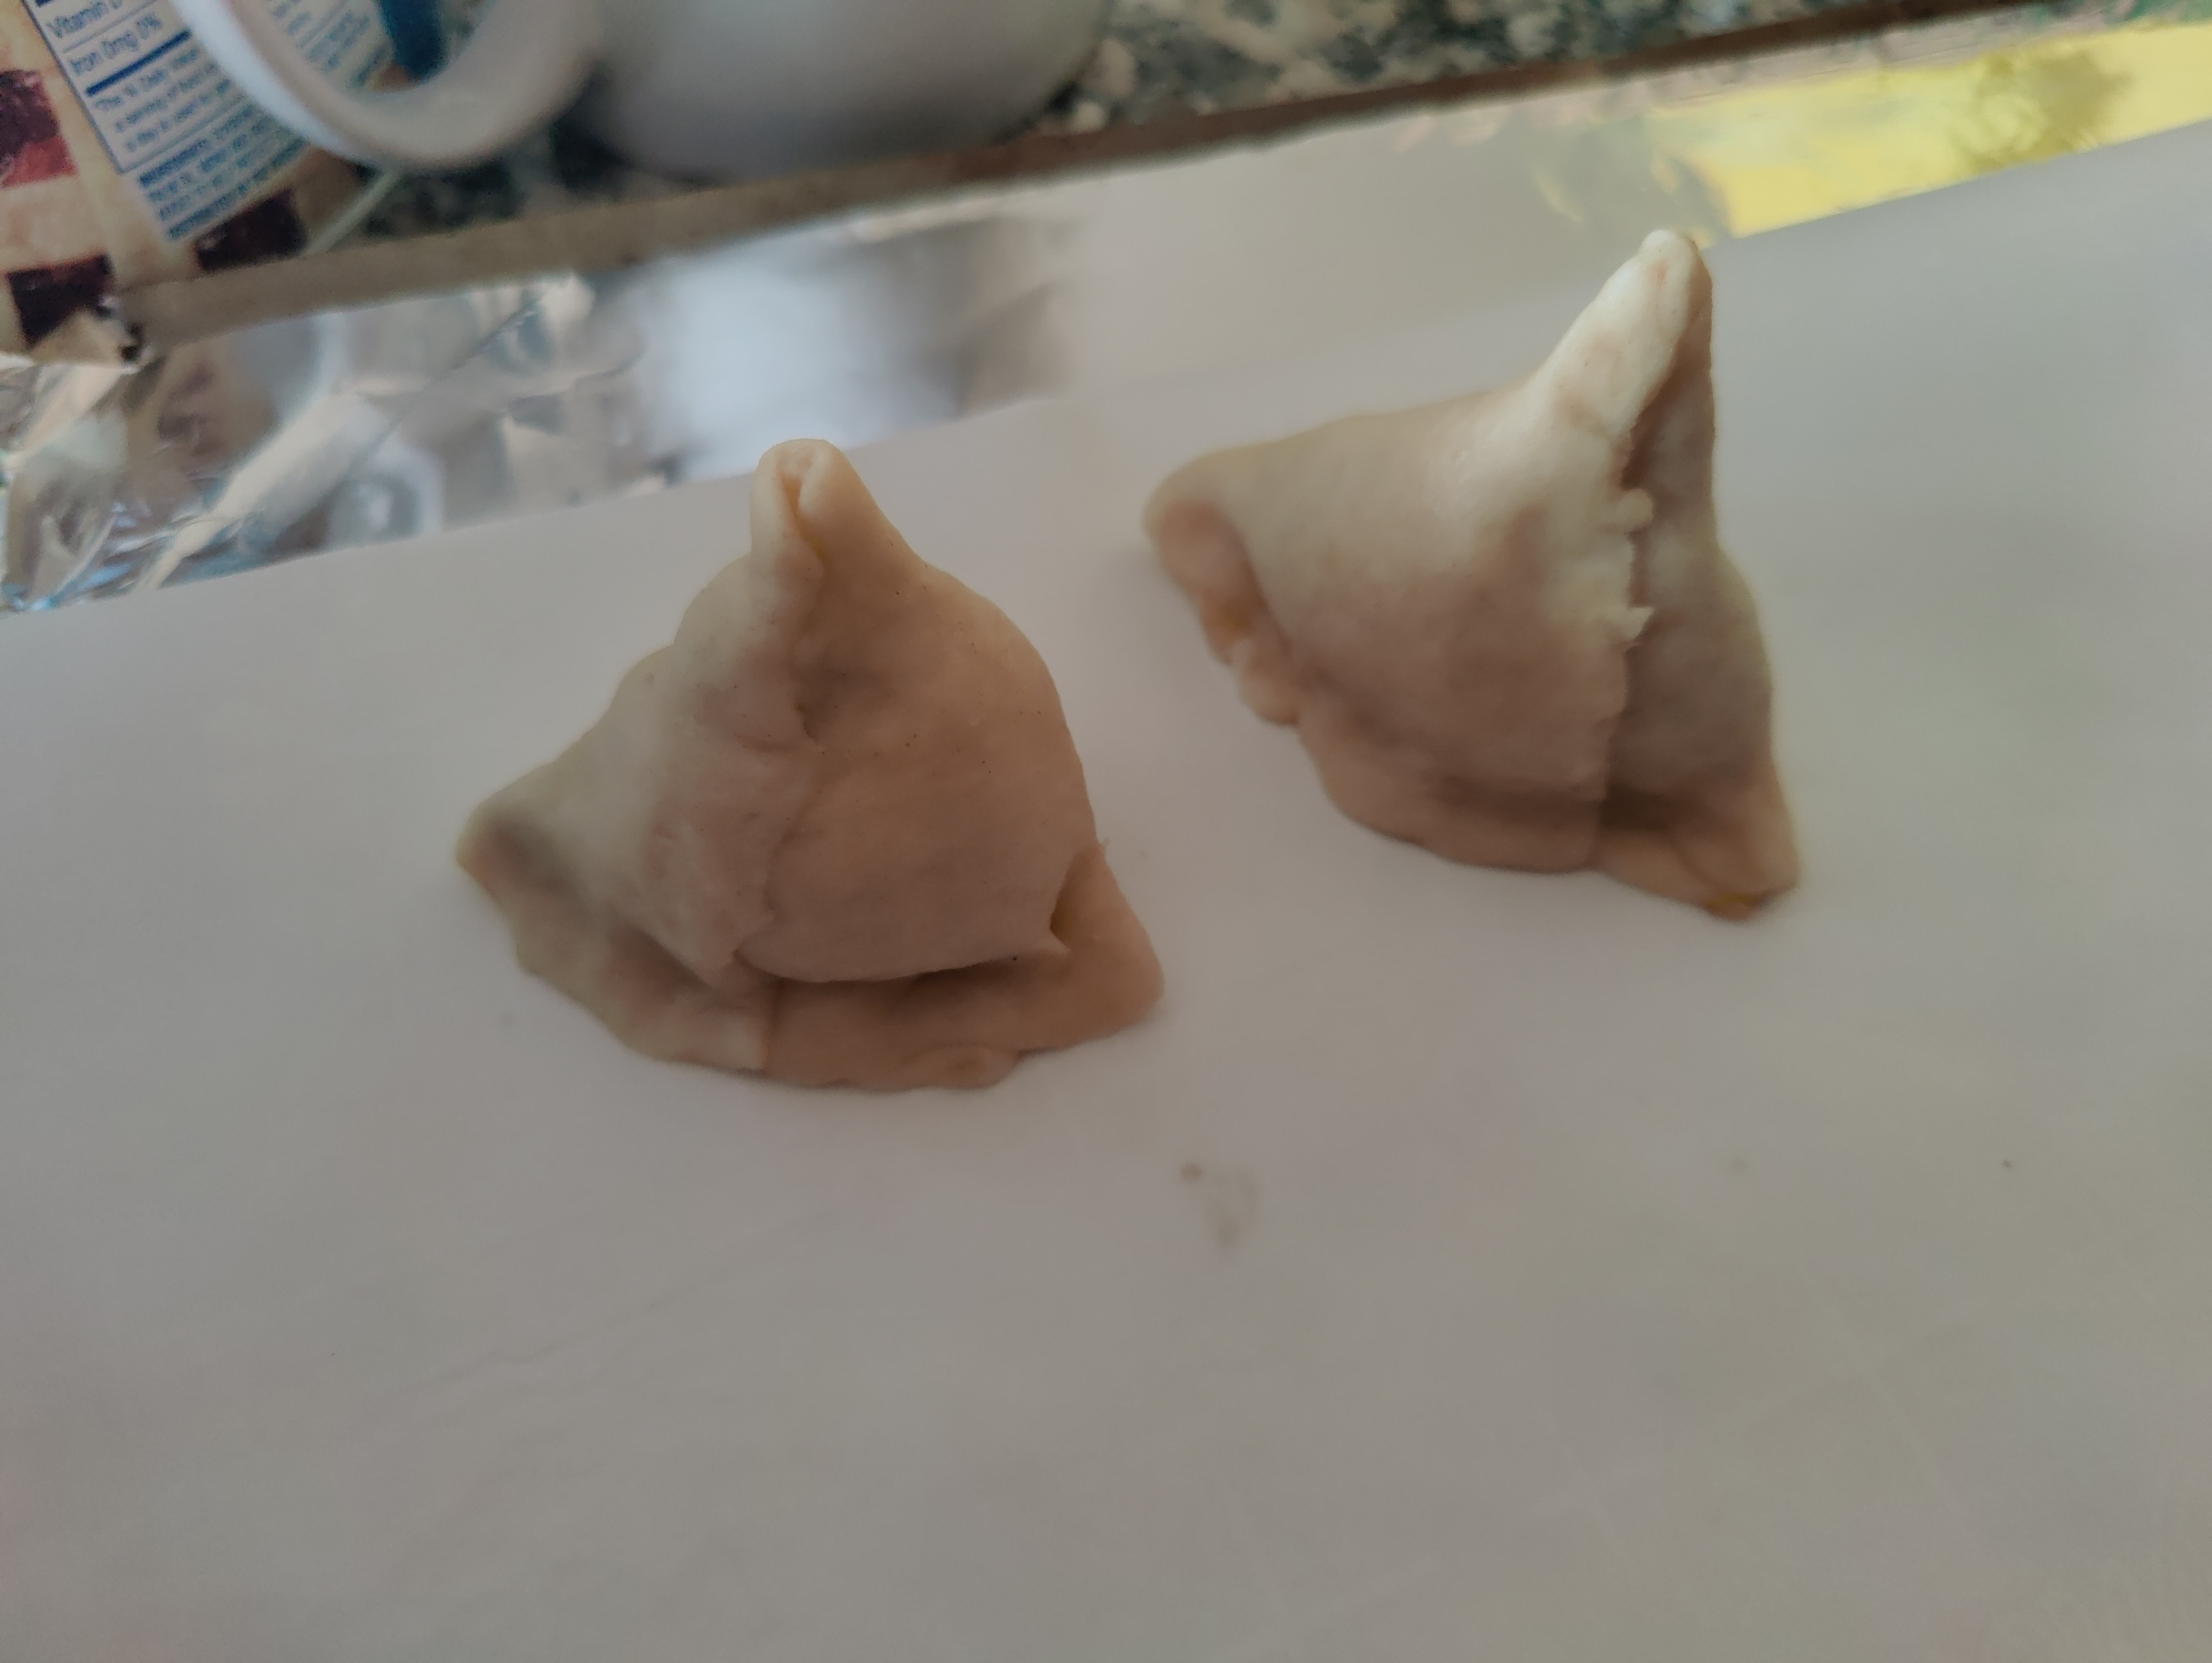
\includegraphics[width=0.5\textwidth]{Samosa/Images/IMG_20231230_143903.jpg}
  \caption{Placing Samosas on baking sheet.}
  \label{fig:fig1}
\end{figure}

\section*{Notes}
\begin{enumerate}
    \item This recipe came out a bit spicy/salty, so people with sensitive pallates might want to reduce the amount of salt and spices.
    \item Raisins and peanuts can be added. I personally do not like raisins in the Samosa.
\end{enumerate}

\begin{figure}[H]
  \centering
  \includegraphics[width=0.7\textwidth]{Samosa/Images/IMG_20231230_141432.jpg}
  \caption{My grandma making the dough}
  \label{fig:fig1}
\end{figure}

